\documentclass[a4paper,10pt,twocolumn]{extarticle}
\usepackage[T1]{fontenc}
%\usepackage[utf8]{inputenc}
\usepackage{lmodern}
\usepackage[francais]{babel}
\usepackage{textcomp}
\usepackage[top=2cm,bottom=2cm,left=2cm,right=2cm]{geometry}
\usepackage{amsmath}
\usepackage{amssymb}
\usepackage{mathrsfs}
\usepackage{float}
\usepackage{icomma}
\usepackage{gensymb}
\usepackage{graphicx}
\usepackage{subcaption}
\usepackage[font=sf, labelfont={sf,bf}, margin=1cm]{caption}
\usepackage[french,onelanguage,ruled,lined]{algorithm2e} % pour pseudo code
\usepackage{array}
\usepackage{titlesec, fontspec, titling}

% Specify different font for section headings
\newfontfamily\headingfont[]{GillSans}
\titleformat*{\section}{\LARGE\headingfont}
\titleformat*{\subsection}{\Large\headingfont}
\titleformat*{\subsubsection}{\large\headingfont}
\renewcommand{\maketitlehooka}{\headingfont}

\pretitle{\begin{flushleft}\fontsize{22}{18}}
\posttitle{\par\end{flushleft}\vskip 0.5em}
\preauthor{\begin{flushleft}\Large \lineskip 0.5em}
\postauthor{\par\end{flushleft}}
%\predate{\begin{flushleft}\large}
%\postdate{\par\end{flushleft}}
\setlength{\droptitle}{-1cm}
\title{\textsf{Implémantation d’un système de détection et de reconnaissance faciale}}
\author{Alexandre Bonhomme\\ {\normalsize Université Paul Sabatier, Toulouse}\\
Florent Maufras\\ {\normalsize EFREI, Paris}\\
Timothée Planté\\ {\normalsize EISTI, Pau}\\}% \small{BONA20128906}}
\date{}

\begin{document}
\maketitle
\section{Introduction}
Le but de notre projet est de prendre en entrée une image comportant un visage d'en faire la détection sur l'image puis d'en tester la reconnaissance sur une base de donnée.

Au final toute image en entrée devrait mener vers un résultat indiquant si le visage qu'elle comporte est reconnu parmi les visages appris par le modèle que l'on a entraîné sur un nombre $x$ d'individu.

\section{Algorithmes mis en oeuvre}
\subsection{K plus proches voisins et Fenêtres de Parzen}
L'algorithme KNN correspond à l'algorithme recherchant les K plus proches voisins (nearest neighbor) et qui permet de classifier en fonction de la classe majoritaire dans ces K voisins sélectionnés.

L'entraînement d'un tel algorithme correspond à l'apprentissage simple des données de l'ensemble d'entraînement. Pour tout nouvel élément test entrant il nous suffit alors de chercher les K plus proches voisins tiré de l'ensemble d'entraînement et d'attribuer comme classe la classe la plus représentée dans son voisinage.
\begin{figure}[H]
  \begin{center}
    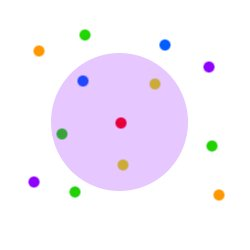
\includegraphics[width=100pt]{images_rapport/KNN.png}
    \caption{K Plus Proches Voisins}
    \label{fig:knn}
  \end{center}
\end{figure}
Dans cet exemple le point de test (point rouge) va recevoir comme prédiction de classe la classe jaune car c'est elle la plus présente dans les K = 4 voisins les plus proches (zone de voisinage de ce point mis en évidence par le disque). Le disque ici n'est que représentatif pour mettre en évidence les voisins. Les points voisins pouvant être à une distance plus ou moins importantes de notre point test.

\subsubsection{Extension avec les fenêtres de Parzen}
L'application que l'on a fait ici de Parzen nous permet ici de rajouter un poids à nos point. Plus un point sera distant du point à l'étude plus sont poids sera faible. Cela est calculé à partir d'une gaussienne centrée sur le point à l'étude et d'une largeur fixé par sigma, sigma dans notre cas est fixé par l'utilisateur.

\subsection{Réseau de Neurones}
L'algorithme du réseau de neurones (Neural Networks) est un modèle qui comporte plusieurs couches et l'entraînement d'un tel système est la tendance à réduire la perte/l'erreur à l'aide de plusieurs itérations. On part d'un état avec des poids définis aléatoirement et on tend alors par une réduction des erreurs à chaque itération vers un état d'apprentissage de notre modèle.
\begin{figure}[H]
  \begin{center}
    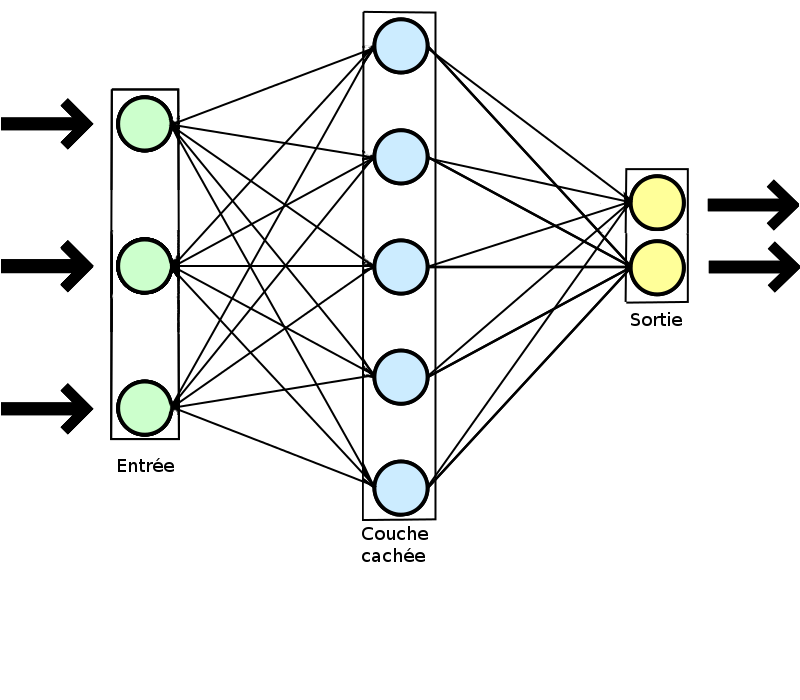
\includegraphics[width=220pt]{images_rapport/Neural_network.png}
    \caption{Réseau de neurones}
    \label{fig:nnet}
  \end{center}
\end{figure}
La réduction de l'erreur revient à la minimisation du risque empirique et la réduction de ce dernier peut-être réalisé de diverses manières :
\begin{description}
  \item[back propagation] consiste en un une propagation de la correction lié à l'erreur depuis la sortie du système vers l'entrée
  \item[feed forward] consiste en une propagation de l'erreur depuis l'entrée vers la sortie
\end{description}

\section{Ensembles de données utilisés}
\subsection{Description}
Nos données sont découpées en deux ensemble : l'ensemble ORL et l'ensemble LFW.  Ces ensembles d'images ont été tiré de base de données d'institut.

Dans le cas du jeu de donnée ORL, l'institut a prit diverses photographies en noir et blanc d’individus avec différentes postures et ce sur plusieurs années pour chacun. Ces clichés sont enregistrés au format pgm.

Pour le second jeu de données, LFW, il s'agit de photographies tirées d'internet et sur lesquels un traitement de détection de visage (Viola et Jones) a été appliqué. Il récupérait alors les visages ainsi repéré en élargissant le cadre autour du visage. Toutes ces images sont en couleurs et au format jpg.

\subsection{Prétraitements}
Toutes les images sont alors traité et ce de façon différente en fonction de l'ensemble de données depuis lequel on la sélectionne. 

Une photographie en couleur, de l'ensemble LFW, sera tout d'abord transformée en une image en niveau de gris puis ensuite on recadra toutes les images selon une taille unique sur toutes les photographies et ce autour des visages. La taille unique est définie par la sélection des maximum observés selon la largeur et la hauteur des cadres obtenus lors de la détection des visages. En effet lors de la détection du visage nous obtenons un encadrement de ce dernier en fonction d'une position, d'une hauteur et d'une largeur.
\begin{figure}[H]
        \centering
        \begin{subfigure}[b]{110pt}
                \centering
                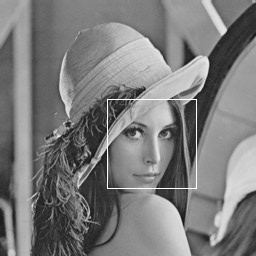
\includegraphics[width=110pt]{images_rapport/lena.png}
                \caption{Image initiale}
                \label{fig:lena}
        \end{subfigure}
        \begin{subfigure}[b]{110pt}
                \centering
                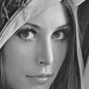
\includegraphics[width=60pt]{images_rapport/lena_face.png}
                \caption{Visage extrait}
                \label{fig:lena_face}
        \end{subfigure}
        \caption{Détection d'un visage par l'algorithme de Viola et Jones \cite{viola01}}
\end{figure}
La transformation alors commune à toutes les images est la vectorisation (\ref{fig:vectorisation}) de ces dernières. Cela revient à passer d'une image matricielle à une image sous forme d'un vecteur selon un des deux axes de la matrice. L'axe choisit est celui des lignes.
\begin{figure}[H]
  \begin{center}
    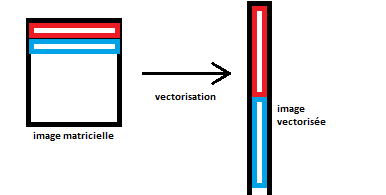
\includegraphics[width=220pt]{images_rapport/vectorisation.png}
    \caption{Vectorisation d'une image}
    \label{fig:vectorisation}
  \end{center}
\end{figure}

\section{Résultats}

\section{}
Un des premiers points spécifiques à notre projet et le fait que ce dernier a été réalisé par une équipe de trois personnes ayant suivi des formations différentes. Nous n'avions pas les même disponibilités non plus pour avancer le projet du fait que nous étions inscris à des cours différents aussi. Cette raison a mené à la mise en place d'une gestionnaire de version avec une centralisation via un site web qui offre ce service : https://bitbucket.org/
Ceci à donc rajouter une difficulté au projet qui était la gestion de l'équipe et la répartition des tâches au sein de cette dernière. L'usage d'un logiciel tel que Git pour gérer les versions en local et via aussi la passerelle distante.

L'usage du python était aussi une des difficultés auquel nous avons voulu nous confronté étant donné que nous avons tous trois découvert ce langage au cours des derniers mois nous voulions essayé de le pratiquer dans en longueur au cours de ce projet.

Le sujet lui-même représente une difficulté quant à la recherche d'un bon résultat étant donné qu'encore à ce jour des entreprises et chercheurs travaillent encore au développement et à l'amélioration de système de reconnaissance faciale car aucun système n'est encore réellement fiable dans ce domaine.

\section{Conclusion}


\begin{thebibliography}{9}
\bibitem{viola01}
  \bsc{Viola P. and Jones M.}, 
  \emph{Rapid object detection using a boosted cascade of simple features}.
  Computer Vision and Pattern Recognition,
  2001.
\bibitem{turk91}
  \bsc{Turk M. and Pentland A.}, 
  \emph{Eigenfaces for recognition}.
  J. Cognitive Neuroscience,
  1991.  
  

\end{thebibliography}
\end{document}
